\documentclass[twoside]{book}

% Packages required by doxygen
\usepackage{fixltx2e}
\usepackage{calc}
\usepackage{doxygen}
\usepackage[export]{adjustbox} % also loads graphicx
\usepackage{graphicx}
\usepackage[utf8]{inputenc}
\usepackage{makeidx}
\usepackage{multicol}
\usepackage{multirow}
\PassOptionsToPackage{warn}{textcomp}
\usepackage{textcomp}
\usepackage[nointegrals]{wasysym}
\usepackage[table]{xcolor}

% Font selection
\usepackage[T1]{fontenc}
\usepackage[scaled=.90]{helvet}
\usepackage{courier}
\usepackage{amssymb}
\usepackage{sectsty}
\renewcommand{\familydefault}{\sfdefault}
\allsectionsfont{%
  \fontseries{bc}\selectfont%
  \color{darkgray}%
}
\renewcommand{\DoxyLabelFont}{%
  \fontseries{bc}\selectfont%
  \color{darkgray}%
}
\newcommand{\+}{\discretionary{\mbox{\scriptsize$\hookleftarrow$}}{}{}}

% Page & text layout
\usepackage{geometry}
\geometry{%
  a4paper,%
  top=2.5cm,%
  bottom=2.5cm,%
  left=2.5cm,%
  right=2.5cm%
}
\tolerance=750
\hfuzz=15pt
\hbadness=750
\setlength{\emergencystretch}{15pt}
\setlength{\parindent}{0cm}
\setlength{\parskip}{3ex plus 2ex minus 2ex}
\makeatletter
\renewcommand{\paragraph}{%
  \@startsection{paragraph}{4}{0ex}{-1.0ex}{1.0ex}{%
    \normalfont\normalsize\bfseries\SS@parafont%
  }%
}
\renewcommand{\subparagraph}{%
  \@startsection{subparagraph}{5}{0ex}{-1.0ex}{1.0ex}{%
    \normalfont\normalsize\bfseries\SS@subparafont%
  }%
}
\makeatother

% Headers & footers
\usepackage{fancyhdr}
\pagestyle{fancyplain}
\fancyhead[LE]{\fancyplain{}{\bfseries\thepage}}
\fancyhead[CE]{\fancyplain{}{}}
\fancyhead[RE]{\fancyplain{}{\bfseries\leftmark}}
\fancyhead[LO]{\fancyplain{}{\bfseries\rightmark}}
\fancyhead[CO]{\fancyplain{}{}}
\fancyhead[RO]{\fancyplain{}{\bfseries\thepage}}
\fancyfoot[LE]{\fancyplain{}{}}
\fancyfoot[CE]{\fancyplain{}{}}
\fancyfoot[RE]{\fancyplain{}{\bfseries\scriptsize Generated by Doxygen }}
\fancyfoot[LO]{\fancyplain{}{\bfseries\scriptsize Generated by Doxygen }}
\fancyfoot[CO]{\fancyplain{}{}}
\fancyfoot[RO]{\fancyplain{}{}}
\renewcommand{\footrulewidth}{0.4pt}
\renewcommand{\chaptermark}[1]{%
  \markboth{#1}{}%
}
\renewcommand{\sectionmark}[1]{%
  \markright{\thesection\ #1}%
}

% Indices & bibliography
\usepackage{natbib}
\usepackage[titles]{tocloft}
\setcounter{tocdepth}{3}
\setcounter{secnumdepth}{5}
\makeindex

% Hyperlinks (required, but should be loaded last)
\usepackage{ifpdf}
\ifpdf
  \usepackage[pdftex,pagebackref=true]{hyperref}
\else
  \usepackage[ps2pdf,pagebackref=true]{hyperref}
\fi
\hypersetup{%
  colorlinks=true,%
  linkcolor=blue,%
  citecolor=blue,%
  unicode%
}

% Custom commands
\newcommand{\clearemptydoublepage}{%
  \newpage{\pagestyle{empty}\cleardoublepage}%
}

\usepackage{caption}
\captionsetup{labelsep=space,justification=centering,font={bf},singlelinecheck=off,skip=4pt,position=top}

%===== C O N T E N T S =====

\begin{document}

% Titlepage & ToC
\hypersetup{pageanchor=false,
             bookmarksnumbered=true,
             pdfencoding=unicode
            }
\pagenumbering{alph}
\begin{titlepage}
\vspace*{7cm}
\begin{center}%
{\Large Lin\+Alg }\\
\vspace*{1cm}
{\large Generated by Doxygen 1.8.13}\\
\end{center}
\end{titlepage}
\clearemptydoublepage
\pagenumbering{roman}
\tableofcontents
\clearemptydoublepage
\pagenumbering{arabic}
\hypersetup{pageanchor=true}

%--- Begin generated contents ---
\chapter{Class Index}
\section{Class List}
Here are the classes, structs, unions and interfaces with brief descriptions\+:\begin{DoxyCompactList}
\item\contentsline{section}{\hyperlink{classMatrix}{Matrix$<$ T $>$} \\*Class template of a matrix to make linear algebra task (hopefully) more friendly }{\pageref{classMatrix}}{}
\end{DoxyCompactList}

\chapter{File Index}
\section{File List}
Here is a list of all documented files with brief descriptions\+:\begin{DoxyCompactList}
\item\contentsline{section}{\hyperlink{my__matrix_8hpp}{my\+\_\+matrix.\+hpp} }{\pageref{my__matrix_8hpp}}{}
\end{DoxyCompactList}

\chapter{Class Documentation}
\hypertarget{classMatrix}{}\doxysection{Matrix$<$ T $>$ Class Template Reference}
\label{classMatrix}\index{Matrix$<$ T $>$@{Matrix$<$ T $>$}}
\doxysubsection*{Public Member Functions}
\begin{DoxyCompactItemize}
\item 
\mbox{\Hypertarget{classMatrix_a0e344d342fe0ad5b208c69f9aa909306}\label{classMatrix_a0e344d342fe0ad5b208c69f9aa909306}} 
{\bfseries Matrix} (const uint \&row, const uint \&col)
\item 
\mbox{\Hypertarget{classMatrix_acb7869d94f5e02b024a0d39d03ec78bd}\label{classMatrix_acb7869d94f5e02b024a0d39d03ec78bd}} 
{\bfseries Matrix} (const uint \&row, const uint \&col, T matrix\+\_\+element)
\item 
\mbox{\Hypertarget{classMatrix_ad9291e60f6af703b79de72d8bcfa777b}\label{classMatrix_ad9291e60f6af703b79de72d8bcfa777b}} 
{\bfseries Matrix} (std\+::initializer\+\_\+list$<$ std\+::vector$<$ T $>$$>$ init\+\_\+list)
\item 
\mbox{\Hypertarget{classMatrix_aace9a20f83d726ffb813fe40ea16bf84}\label{classMatrix_aace9a20f83d726ffb813fe40ea16bf84}} 
{\bfseries Matrix} (std\+::vector$<$ std\+::vector$<$ T $>$$>$)
\item 
\mbox{\Hypertarget{classMatrix_a2b6e9de6b55a40317911aa6c7adfa72a}\label{classMatrix_a2b6e9de6b55a40317911aa6c7adfa72a}} 
{\bfseries Matrix} (const uint \&row, const uint \&col, const double \&mean, const double \&sd)
\item 
\mbox{\Hypertarget{classMatrix_a42241ef961d7b919f3ec952e16ae0b55}\label{classMatrix_a42241ef961d7b919f3ec952e16ae0b55}} 
std\+::vector$<$ std\+::vector$<$ T $>$ $>$ {\bfseries get\+\_\+matrix} () const
\item 
\mbox{\Hypertarget{classMatrix_afdc70f8e656996481f5a6b970189c64b}\label{classMatrix_afdc70f8e656996481f5a6b970189c64b}} 
std\+::vector$<$ T $>$ {\bfseries diag} (const int id) const
\item 
\mbox{\Hypertarget{classMatrix_a3a9452f46689001f2f262f13d4600ea9}\label{classMatrix_a3a9452f46689001f2f262f13d4600ea9}} 
\mbox{\hyperlink{classMatrix}{Matrix}}$<$ T $>$ {\bfseries operator()} (const uint \&row\+\_\+1, const uint \&row\+\_\+2, const uint \&col\+\_\+1, const uint \&col\+\_\+2)
\item 
\mbox{\Hypertarget{classMatrix_afdf86fadf4ac353f6f32e780a5016c25}\label{classMatrix_afdf86fadf4ac353f6f32e780a5016c25}} 
T {\bfseries dimension} (const uint \&idx) const
\item 
\mbox{\Hypertarget{classMatrix_a8396ba9c5609d2fb1014262fbf172479}\label{classMatrix_a8396ba9c5609d2fb1014262fbf172479}} 
T \& {\bfseries operator()} (const uint \&row\+\_\+idx, const uint \&col\+\_\+idx)
\item 
\mbox{\Hypertarget{classMatrix_ae6ab8af0e5d03eb8fe5f31d037b2e207}\label{classMatrix_ae6ab8af0e5d03eb8fe5f31d037b2e207}} 
T {\bfseries operator()} (const uint \&row\+\_\+idx, const uint \&col\+\_\+idx) const
\item 
\mbox{\Hypertarget{classMatrix_aa0347b091217f8ea2a928efd860d4d26}\label{classMatrix_aa0347b091217f8ea2a928efd860d4d26}} 
double {\bfseries determinant} ()
\item 
\mbox{\Hypertarget{classMatrix_abb26547343d449fbedc5bd3b24120927}\label{classMatrix_abb26547343d449fbedc5bd3b24120927}} 
void {\bfseries Tr} ()
\item 
\mbox{\Hypertarget{classMatrix_af531b530699d08cb75b3ceabf22618fb}\label{classMatrix_af531b530699d08cb75b3ceabf22618fb}} 
T {\bfseries det} ()
\item 
\mbox{\Hypertarget{classMatrix_afe220c54165e01d7b3d528c8425aff07}\label{classMatrix_afe220c54165e01d7b3d528c8425aff07}} 
\mbox{\hyperlink{classMatrix}{Matrix}}$<$ T $>$ {\bfseries gauss\+\_\+elimination} ()
\end{DoxyCompactItemize}
\doxysubsection*{Friends}
\begin{DoxyCompactItemize}
\item 
\mbox{\Hypertarget{classMatrix_a1dc63135b1211215f22dd9f691eaf1f9}\label{classMatrix_a1dc63135b1211215f22dd9f691eaf1f9}} 
{\footnotesize template$<$typename U $>$ }\\\mbox{\hyperlink{classMatrix}{Matrix}}$<$ U $>$ {\bfseries operator$\ast$} (const \mbox{\hyperlink{classMatrix}{Matrix}}$<$ U $>$ \&a, const U \&scalar)
\item 
\mbox{\Hypertarget{classMatrix_abe73619c6b45315d7efd6a2074ed71bd}\label{classMatrix_abe73619c6b45315d7efd6a2074ed71bd}} 
{\footnotesize template$<$typename U $>$ }\\std\+::ostream \& {\bfseries operator$<$$<$} (std\+::ostream \&out, const \mbox{\hyperlink{classMatrix}{Matrix}}$<$ U $>$ \&a)
\end{DoxyCompactItemize}


\doxysubsection{Detailed Description}
\subsubsection*{template$<$typename T$>$\newline
class Matrix$<$ T $>$}



Definition at line 11 of file my\+\_\+matrix.\+hpp.



The documentation for this class was generated from the following file\+:\begin{DoxyCompactItemize}
\item 
my\+\_\+matrix.\+hpp\end{DoxyCompactItemize}

\chapter{File Documentation}
\hypertarget{my__matrix_8hpp}{}\section{my\+\_\+matrix.\+hpp File Reference}
\label{my__matrix_8hpp}\index{my\+\_\+matrix.\+hpp@{my\+\_\+matrix.\+hpp}}
{\ttfamily \#include $<$vector$>$}\newline
{\ttfamily \#include $<$initializer\+\_\+list$>$}\newline
{\ttfamily \#include $<$iostream$>$}\newline
{\ttfamily \#include $<$algorithm$>$}\newline
{\ttfamily \#include $<$iterator$>$}\newline
{\ttfamily \#include $<$numeric$>$}\newline
{\ttfamily \#include $<$random$>$}\newline
Include dependency graph for my\+\_\+matrix.\+hpp\+:\nopagebreak
\begin{figure}[H]
\begin{center}
\leavevmode
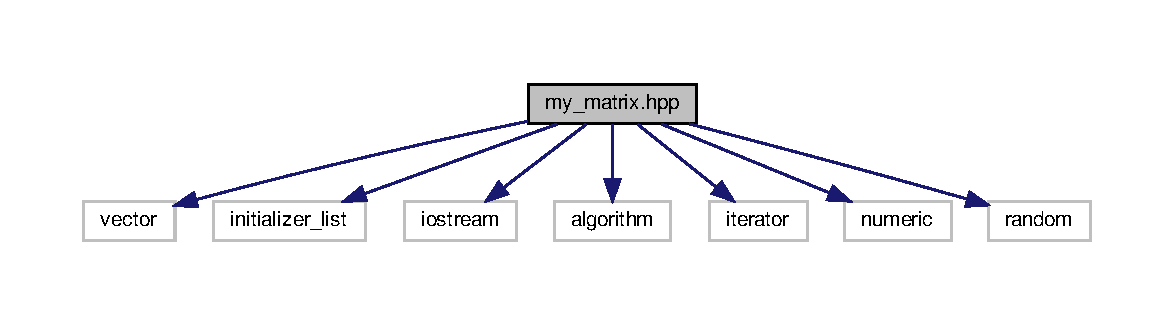
\includegraphics[width=350pt]{my__matrix_8hpp__incl}
\end{center}
\end{figure}
\subsection*{Classes}
\begin{DoxyCompactItemize}
\item 
class \hyperlink{classMatrix}{Matrix$<$ T $>$}
\begin{DoxyCompactList}\small\item\em Class template of a matrix to make linear algebra task (hopefully) more friendly. \end{DoxyCompactList}\end{DoxyCompactItemize}
\subsection*{Functions}
\begin{DoxyCompactItemize}
\item 
\mbox{\Hypertarget{my__matrix_8hpp_abe73619c6b45315d7efd6a2074ed71bd}\label{my__matrix_8hpp_abe73619c6b45315d7efd6a2074ed71bd}} 
{\footnotesize template$<$typename U $>$ }\\std\+::ostream \& {\bfseries operator$<$$<$} (std\+::ostream \&out, const \hyperlink{classMatrix}{Matrix}$<$ U $>$ \&a)
\item 
\mbox{\Hypertarget{my__matrix_8hpp_a1dc63135b1211215f22dd9f691eaf1f9}\label{my__matrix_8hpp_a1dc63135b1211215f22dd9f691eaf1f9}} 
{\footnotesize template$<$typename U $>$ }\\\hyperlink{classMatrix}{Matrix}$<$ U $>$ {\bfseries operator$\ast$} (const \hyperlink{classMatrix}{Matrix}$<$ U $>$ \&a, const U \&scalar)
\item 
\mbox{\Hypertarget{my__matrix_8hpp_a6572630f7652d8e8e26621fd13e5a2a2}\label{my__matrix_8hpp_a6572630f7652d8e8e26621fd13e5a2a2}} 
{\footnotesize template$<$typename T $>$ }\\\hyperlink{classMatrix}{Matrix}$<$ T $>$ {\bfseries operator$\ast$} (const \hyperlink{classMatrix}{Matrix}$<$ T $>$ \&a, const \hyperlink{classMatrix}{Matrix}$<$ T $>$ \&b)
\end{DoxyCompactItemize}


\subsection{Detailed Description}
\begin{DoxyAuthor}{Author}
Andrea Cordone 
\end{DoxyAuthor}

%--- End generated contents ---

% Index
\backmatter
\newpage
\phantomsection
\clearemptydoublepage
\addcontentsline{toc}{chapter}{Index}
\printindex

\end{document}
